\documentclass[spanish,a4paper,12pt,oneside]{extreport}

\usepackage[dvips]{graphicx}
\usepackage[dvips]{epsfig}
\usepackage[T1]{fontenc}
\usepackage[utf8]{inputenc}
\usepackage[spanish]{babel}

\usepackage{multirow}
\usepackage{array}
\usepackage{booktabs}
\usepackage{caption}
\usepackage{float}
\usepackage{graphicx}
\usepackage{subcaption}
\usepackage{hyperref}
\usepackage{xcolor}

\usepackage{titlesec}
\titleformat{\chapter}[block]{\Large\bfseries}{\thechapter.}{0.5em}{}
\titlespacing*{\chapter}{0pt}{20pt}{12pt}

\usepackage[top=2cm, bottom=2cm, left=2cm, right=2cm]{geometry}

\usepackage{listings}

\definecolor{background}{HTML}{EEEEEE}
\definecolor{codeblue}{HTML}{2563EB}

\lstset{
    basicstyle=\small\ttfamily,
    breaklines=true,
    frame=single,
    backgroundcolor=\color{background},
    showstringspaces=false,
    keepspaces=true,
    columns=fullflexible,
    language=Python,
    keywordstyle=\color{codeblue},
    commentstyle=\color{gray},
    stringstyle=\color{teal},
    extendedchars=true,
    inputencoding=utf8,
    literate=
      {á}{{\'{a}}}1 {é}{{\'{e}}}1 {í}{{\'{i}}}1 {ó}{{\'{o}}}1 {ú}{{\'{u}}}1
      {Á}{{\'{A}}}1 {É}{{\'{E}}}1 {Í}{{\'{I}}}1 {Ó}{{\'{O}}}1 {Ú}{{\'{U}}}1
      {ñ}{{\~{n}}}1 {Ñ}{{\~{N}}}1
      {ü}{{\"u}}1,
}

\begin{document}

\renewcommand\listtablename{Índice de Tablas}
\renewcommand\listfigurename{Índice de Figuras}

\pagestyle{empty}
\thispagestyle{empty}

\newcommand{\HRule}{\rule{\linewidth}{1mm}}
\setlength{\parindent}{0mm}
\setlength{\parskip}{0mm}

\vspace*{\stretch{0.5}}

\begin{center}
  {\Huge Trabajo Final de Visualización}\\[5mm]
  {\large Máster Universitario en Inteligencia de Datos y Ciberseguridad}
\end{center}

\HRule
\begin{flushright}
        {\Huge Análisis de la desigualdad económica\\en la provincia de Santa Cruz de Tenerife} \\[2.5mm]
        {\Large Francisco Marqués Armas} \\[5mm]
\end{flushright}
\HRule
\vspace*{\stretch{2}}
\begin{center}
  \Large La Laguna, \today
\end{center}

\setlength{\parindent}{5mm}

\pagenumbering{roman}
\pagestyle{plain}

\setcounter{tocdepth}{2}
\tableofcontents

\newpage
\pagenumbering{arabic}
\pagestyle{plain}


% =============================================================================
\chapter{Introducción y descripción del conjunto de datos}
% =============================================================================

\section{Motivación}

La provincia de Santa Cruz de Tenerife presenta una distribución de la renta desigual, ya que municipios turísticos y de servicios conviven con zonas de actividad agrícola o poca actividad económica cuya renta per cápita es significativamente inferior. Este proyecto aplica las técnicas de visualización de datos aprendidas en la asignatura para cuantificar esa desigualdad a través de datos oficiales del Instituto Nacional de Estadística (INE).

\section{Fuentes de datos}

El proyecto emplea cuatro conjuntos de datos:

\begin{table}[H]
\centering
\begin{tabular}{llp{4.5cm}p{4cm}}
\toprule
Dataset & Variable clave & Cobertura & Granularidad \\
\midrule
Renta media neta & OBS\_VALUE (euros/hogar) & 2021--2023 & Sección censal \\
Fuentes de ingresos & Porcentaje por fuente & 2023 & Municipio \\
Actividad económica & Número de trabajadores & 2023 & Municipio por sector \\
Categoría de ocupación & Número de trabajadores & 2023 & Municipio, ocupación y sexo \\
\bottomrule
\end{tabular}
\caption{Conjuntos de datos utilizados. Los cuatro proceden del INE y cubren la provincia de Santa Cruz de Tenerife (código INE: 38).}
\end{table}

\begin{itemize}
  \item Renta media: Atlas de distribución de renta de los hogares (ADRH), indicador de renta neta media por hogar a nivel de sección censal. Permite comparar municipios y analizar la desigualdad intramunicipal.
  \item Fuentes de ingresos: porcentaje de la renta total que procede de sueldos y salarios, pensiones, prestaciones por desempleo, otras prestaciones sociales y otros ingresos.
  \item Actividad económica: distribución de los asalariados por sector CNAE: Agricultura/pesca, Construcción, Industria y Servicios.
  \item Categoría de ocupación: distribución de asalariados por categoría de ocupación (CNO) y sexo, lo que permite estudiar la brecha de género.
\end{itemize}

\section{Preguntas de investigación}

Las visualizaciones se organizan en torno a tres preguntas:

\begin{enumerate}
  \item ?`Cómo se distribuye la renta entre los municipios? ?`Hay diferencias sistemáticas entre islas? ?`Ha evolucionado la brecha en los últimos tres años?
  \item ?`Qué caracteriza económicamente a los municipios ricos y a los pobres? ?`En qué sectores trabajan, qué ingresos reciben y qué ocupaciones predominan en los extremos de la distribución?
  \item ?`Qué desigualdad existe dentro de cada municipio? ?`Qué secciones censales concentran la riqueza y cuáles la pobreza?
\end{enumerate}


% =============================================================================
\chapter{Gramática de gráficos}
% =============================================================================

A continuación se analiza cada visualización generada siguiendo la gramática de gráficos de Wilkinson \cite{wilkinson2005} tal como la implementa Plotnine \cite{plotnine}: datos, mapeos estéticos (aes), geometrías (geom\_*), escalas, coordenadas, facetas y tema.

\section{Lollipop: ranking de municipios por renta media}

\begin{figure}[H]
\centering
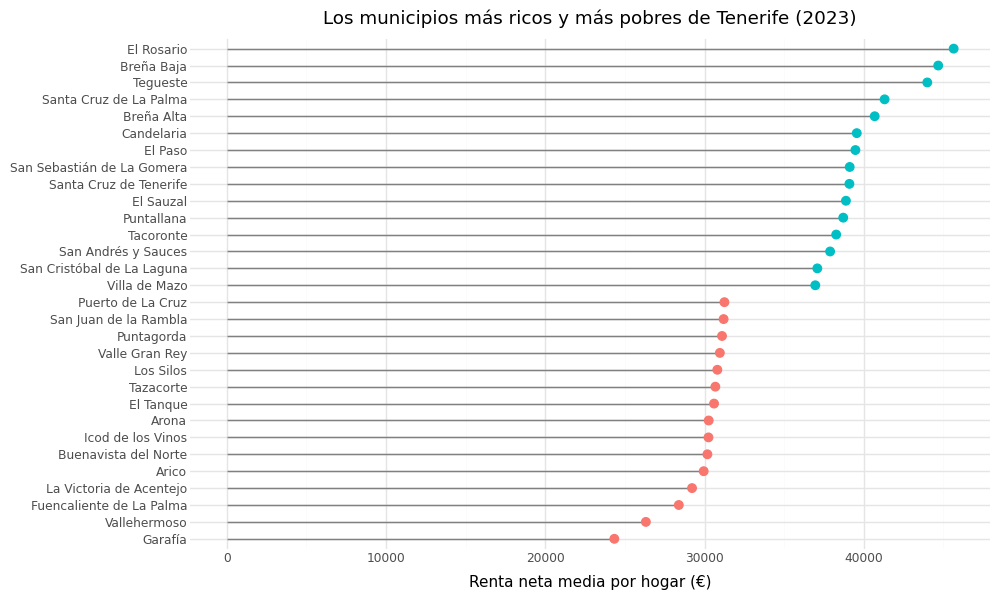
\includegraphics[width=0.82\textwidth]{images/ranking}
\caption{Lollipop de ranking de municipios por renta media neta (2023).}
\end{figure}

\begin{itemize}
  \item Datos: tabla con un registro por municipio; columnas municipio (cadena) y renta\_media (numérico, euros).
  \item Mapeos:
    \begin{itemize}
      \item x = municipio (variable categórica, ordenada por renta de menor a mayor)
      \item y = renta\_media (variable cuantitativa continua)
      \item color = isla (variable categórica nominal; distingue visualmente a qué isla pertenece cada municipio)
    \end{itemize}
  \item Geometrías: geom\_segment (el palo del lollipop, desde y=0 hasta el valor) + geom\_point (la cabeza del lollipop).
  \item Escalas:
    \begin{itemize}
      \item Eje Y: escala continua en euros; etiquetas con separador de miles.
      \item Color: escala discreta cualitativa (cuatro colores, uno por isla).
    \end{itemize}
  \item Coordenadas: coord\_flip() para orientar las barras horizontalmente y hacer legibles los nombres de municipio.
  \item Facetas: ninguna; todos los municipios en un único panel.
  \item Tema: theme\_minimal() con texto del eje Y reducido (size=7) para acomodar 54 etiquetas.
\end{itemize}

El lollipop es preferible al gráfico de barras cuando hay muchas categorías: la línea delgada reduce el ruido visual y la comparación de valores se realiza rápidamente gracias al punto claramente posicionado.

\section{Histograma: distribución de la renta por sección censal}

\begin{figure}[H]
\centering
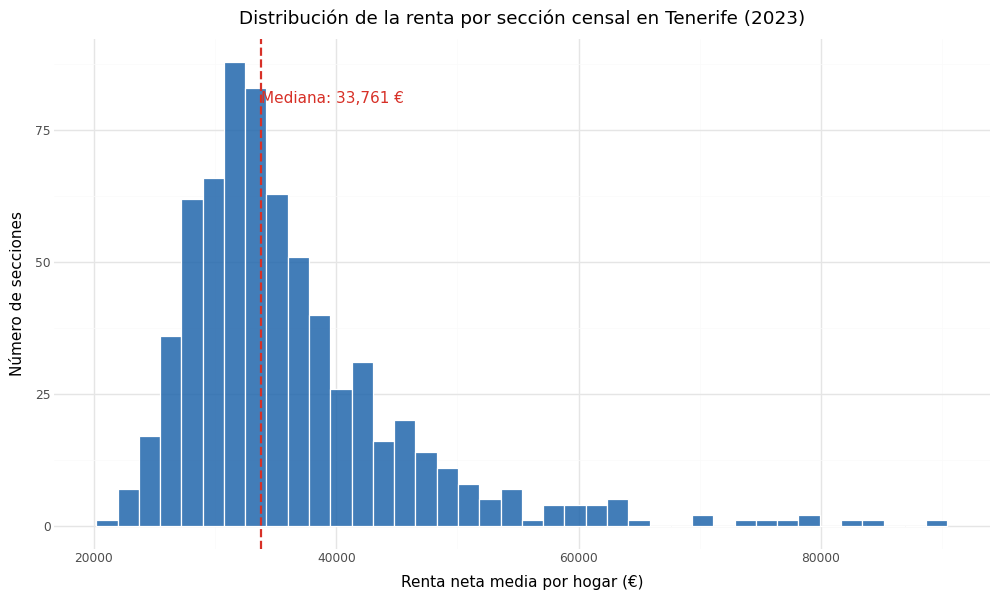
\includegraphics[width=\textwidth]{images/histograma}
\caption{Histograma de distribución de la renta neta por sección censal.}
\end{figure}

\begin{itemize}
  \item Datos: tabla con un registro por sección censal; columna renta\_neta.
  \item Mapeos: x = renta\_neta.
  \item Geometrías: geom\_histogram (bins=40) + geom\_vline para indicar la mediana.
  \item Escalas: eje X continuo en euros; eje Y de frecuencia absoluta.
  \item Coordenadas: cartesianas estándar.
  \item Facetas: ninguna.
  \item Tema: theme\_minimal().
\end{itemize}

El histograma revela la asimetría positiva (cola derecha larga) característica de las distribuciones de renta: la mayoría de las secciones se concentran en la parte baja, con pocas secciones de renta muy alta.

\section{Waterfall: fuentes de ingresos}

\begin{figure}[H]
\centering
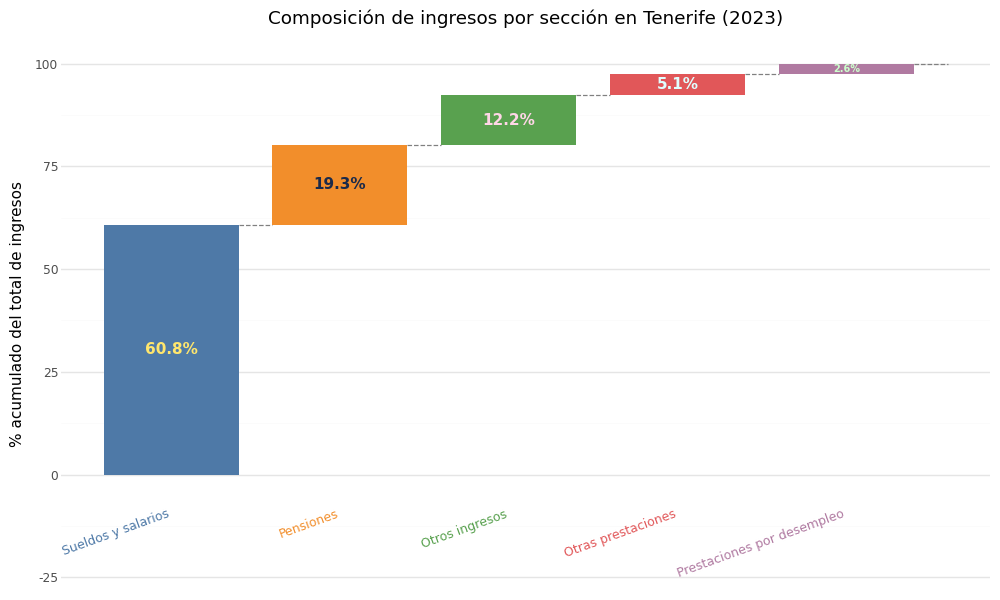
\includegraphics[width=\textwidth]{images/waterfall_fuentes}
\caption{Waterfall de fuentes de ingresos: composición porcentual (2023).}
\end{figure}

\begin{itemize}
  \item Datos: cinco filas, una por fuente de ingresos; columnas fuente y pct (porcentaje del total).
  \item Mapeos: x = fuente (categórica), y = pct, fill = fuente.
  \item Geometrías: geom\_col con las barras apiladas en cascada (waterfall): cada barra comienza donde termina la anterior, de modo que la suma acumulada avanza de izquierda a derecha hasta el 100\%.
  \item Escalas: eje Y en porcentaje; paleta de colores divergente para distinguir fuentes activas (sueldos) de pasivas (pensiones, prestaciones).
  \item Coordenadas: cartesianas.
  \item Facetas: ninguna.
  \item Tema: etiquetas de porcentaje sobre cada barra con geom\_text.
\end{itemize}

\section{Waterfall: distribución por sector de actividad}

\begin{figure}[H]
\centering
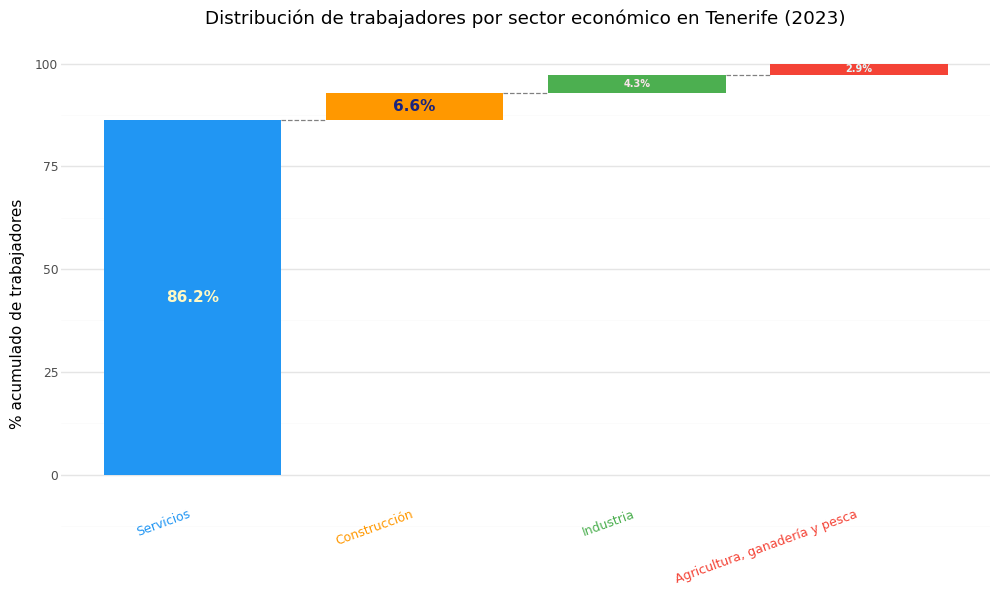
\includegraphics[width=\textwidth]{images/waterfall_actividades}
\caption{Waterfall de distribución de trabajadores por sector de actividad (2023).}
\end{figure}

Mismo esquema que el anterior pero para los cuatro sectores CNAE: Servicios, Industria, Construcción y Agricultura. El sector servicios domina ampliamente (más del 70\% de los asalariados), dato que da contexto a los gráficos de quintiles.

\section{Diverging bar: brecha de género en ocupaciones}

\begin{figure}[H]
\centering
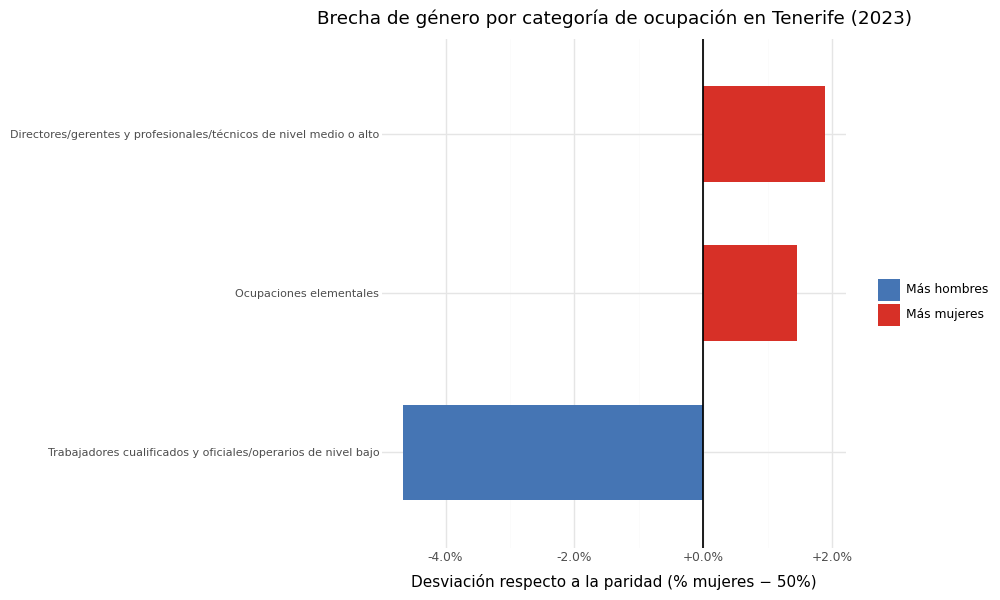
\includegraphics[width=\textwidth]{images/diverging_genero}
\caption{Desviación respecto a la paridad de género (50/50) por categoría de ocupación (2023).}
\end{figure}

\begin{itemize}
  \item Datos: tabla con un registro por categoría de ocupación; columnas ocupacion, desviacion (porcentaje de mujeres menos 50) y mayoria ("Más mujeres" / "Más hombres").
  \item Mapeos:
    \begin{itemize}
      \item x = ocupacion (categórica, ordenada por desviación)
      \item y = desviacion (numérico; negativo = mayoría masculina, positivo = mayoría femenina)
      \item fill = mayoria (dos colores: rojo para mayoría femenina, azul para masculina)
    \end{itemize}
  \item Geometrías: geom\_col + geom\_hline(yintercept=0) para la línea de paridad.
  \item Escalas: eje Y con etiquetas en formato +X.X\% / -X.X\%; escala de color manual con dos valores.
  \item Coordenadas: coord\_flip().
  \item Facetas: ninguna.
  \item Tema: leyenda integrada en el gráfico; texto del eje Y reducido.
\end{itemize}

El diverging bar es el tipo de gráfico más adecuado para mostrar desviaciones respecto a un punto de referencia (aquí, la paridad perfecta al 50\%). Permite ver de un vistazo qué categorías están feminizadas o masculinizadas.


\section{Box plots: desigualdad intramunicipal por isla}

\begin{itemize}
  \item Datos: un registro por sección censal con columnas municipio e isla. Se filtra por isla y se genera un PNG independiente por isla.
  \item Mapeos: x = municipio (categórica, ordenada por mediana), y = renta\_neta.
  \item Geometrías: geom\_boxplot con outlier\_size=0.8 (puntos pequeños para los valores atípicos).
  \item Escalas: eje Y continuo en euros.
  \item Coordenadas: coord\_flip().
  \item Facetas: ninguna (se generan cuatro archivos separados en lugar de un facet\_wrap).
  \item Tema: theme\_minimal() sin leyenda; altura del gráfico escalada automáticamente según el número de municipios de la isla.
\end{itemize}

Generar un PNG por isla en lugar de un único gráfico con facetas permite adaptar la escala vertical a cada isla y evitar que los municipios de islas pequeñas queden aplastados.

\begin{figure}[H]
\centering
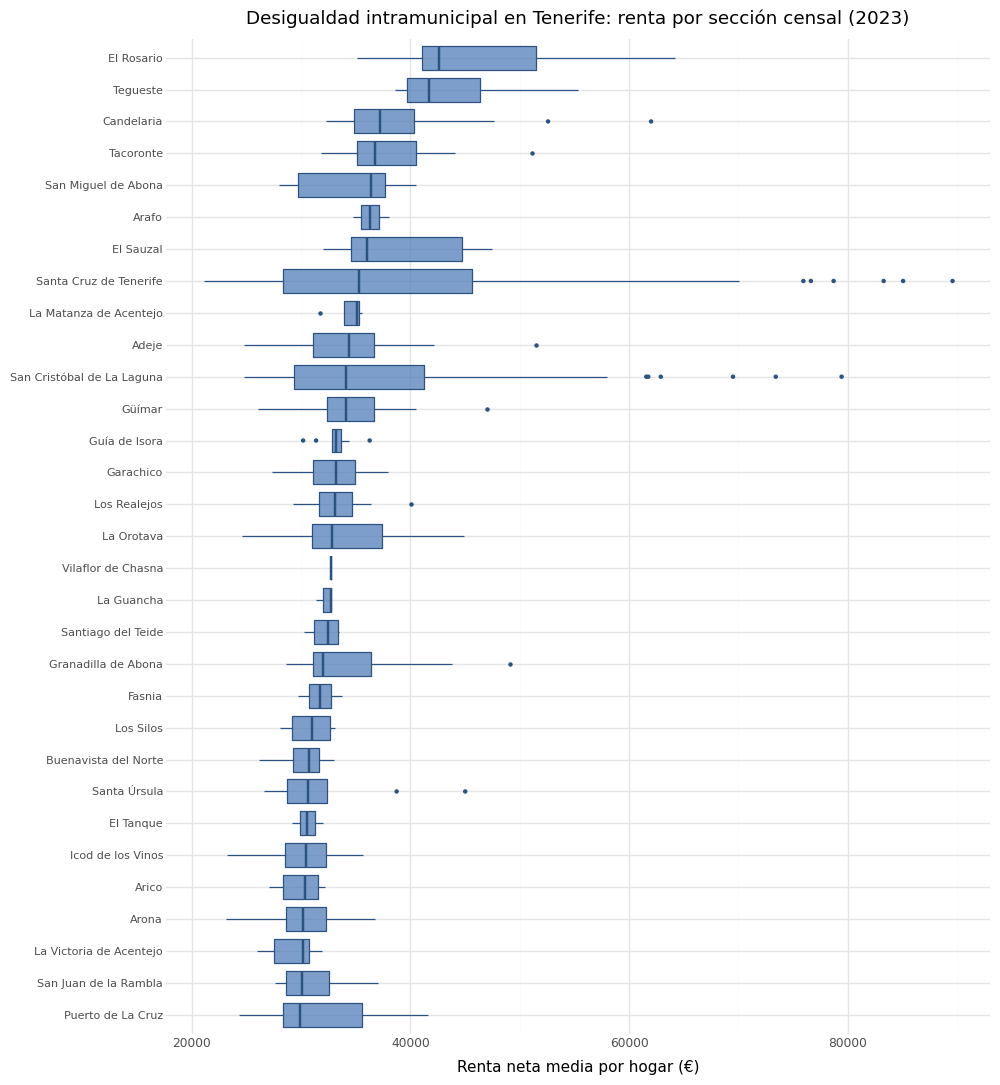
\includegraphics[width=\textwidth]{images/boxplot_tenerife}
\caption{Desigualdad intramunicipal en Tenerife: renta por sección censal (2023).}
\end{figure}

\begin{figure}[H]
\centering
\begin{subfigure}[b]{0.48\textwidth}
  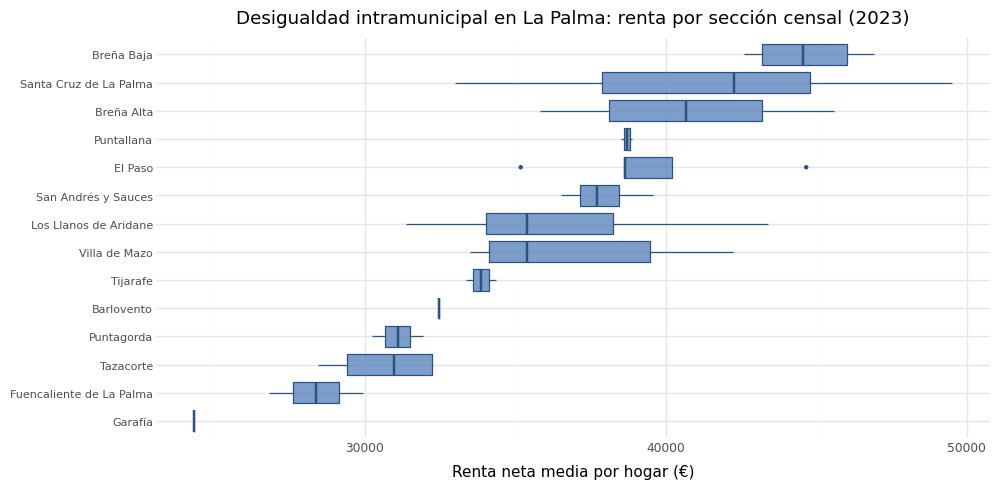
\includegraphics[width=\textwidth]{images/boxplot_palma}
  \caption{La Palma}
\end{subfigure}
\hfill
\begin{subfigure}[b]{0.48\textwidth}
  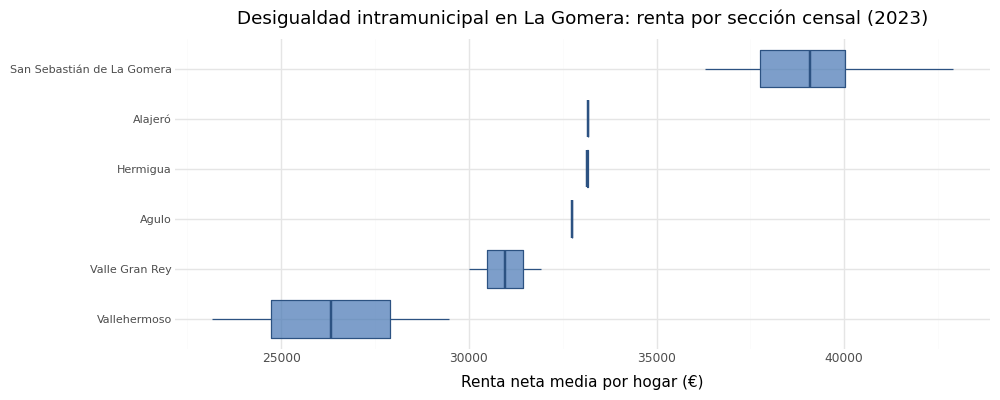
\includegraphics[width=\textwidth]{images/boxplot_gomera}
  \caption{La Gomera}
\end{subfigure}
\\[6pt]
\begin{subfigure}[b]{0.48\textwidth}
  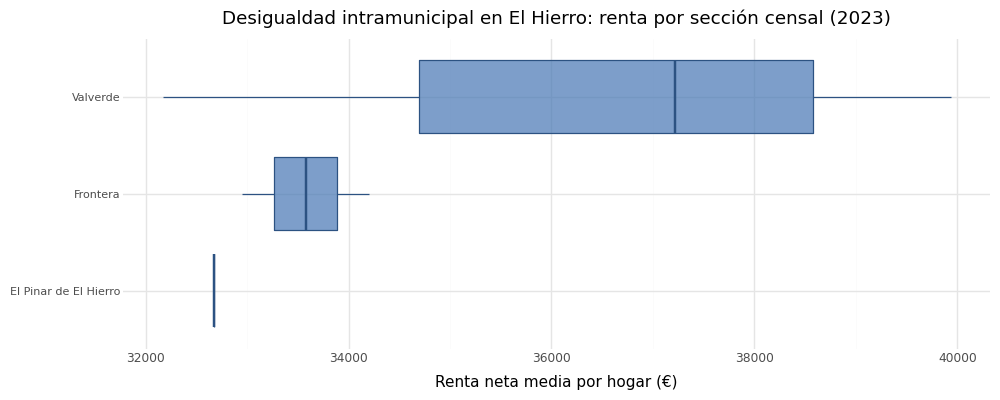
\includegraphics[width=\textwidth]{images/boxplot_hierro}
  \caption{El Hierro}
\end{subfigure}
\caption{Desigualdad intramunicipal en las islas menores: renta por sección censal (2023).}
\end{figure}

\section{Scatter: estudios elementales vs. renta}

\begin{figure}[H]
\centering
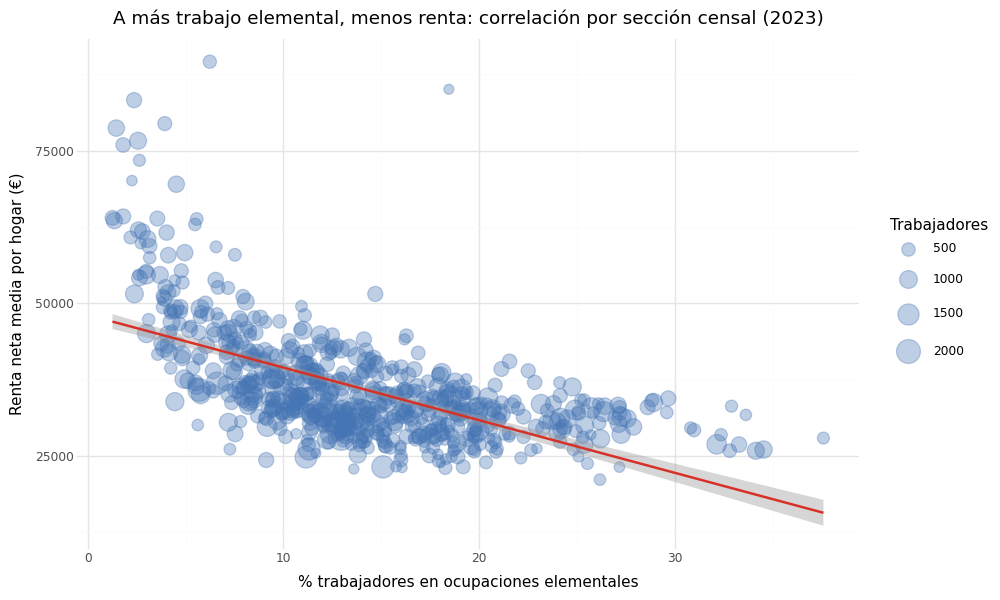
\includegraphics[width=\textwidth]{images/scatter}
\caption{Relación entre porcentaje de trabajadores con nivel elemental y renta media municipal (2023).}
\end{figure}

\begin{itemize}
  \item Datos: un registro por municipio; columnas pct\_elementales (porcentaje de trabajadores con nivel formativo elemental) y renta\_neta (renta media).
  \item Mapeos: x = pct\_elementales, y = renta\_neta, label = municipio (para identificar puntos extremos).
  \item Geometrías: geom\_point + geom\_smooth(method='lm') (regresión lineal) + geom\_text para las etiquetas.
  \item Escalas: ambos ejes continuos; eje X en porcentaje.
  \item Coordenadas: cartesianas.
  \item Facetas: ninguna.
  \item Tema: theme\_minimal().
\end{itemize}

La correlación negativa esperada (a mayor porcentaje de trabajadores con estudios elementales, menor renta media) valida el supuesto narrativo del proyecto.

\section{Grouped bar: distribución de actividad por quintil de renta}

\begin{figure}[H]
\centering
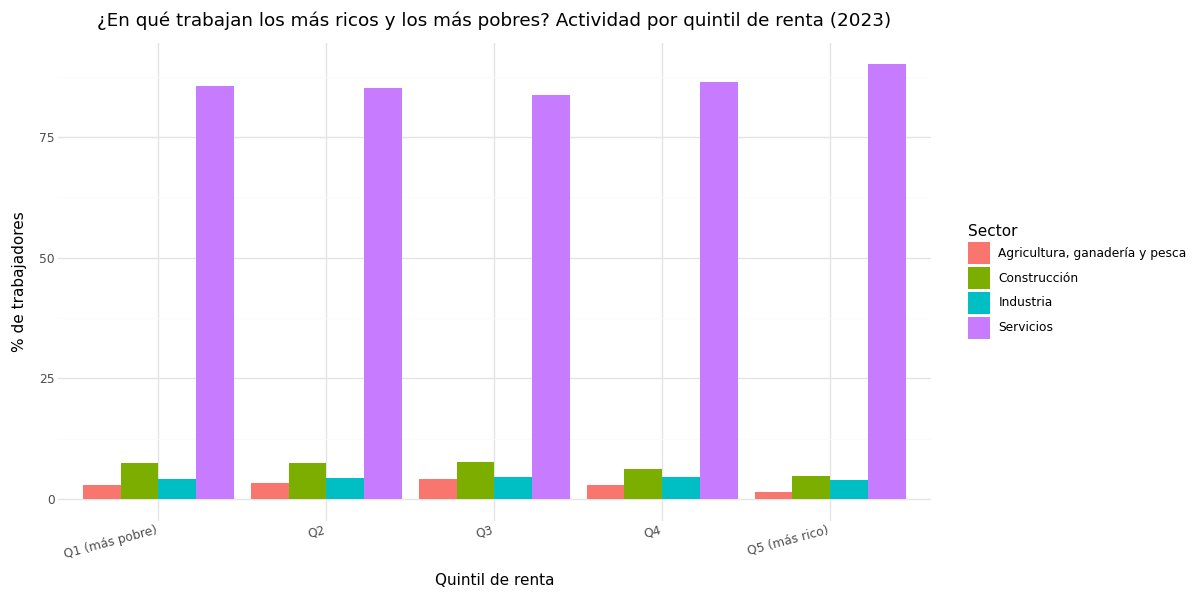
\includegraphics[width=\textwidth]{images/grouped_actividad}
\caption{Distribución de trabajadores por sector de actividad y quintil de renta (2023).}
\end{figure}

\begin{itemize}
  \item Datos: tabla con columnas quintil (1--5), actividad (sector CNAE) y pct (porcentaje de trabajadores).
  \item Mapeos: x = quintil, y = pct, fill = actividad.
  \item Geometrías: geom\_col(position='dodge') (barras agrupadas, no apiladas).
  \item Escalas: eje Y en porcentaje; paleta de colores cualitativos para los cuatro sectores.
  \item Coordenadas: cartesianas; eje X discreto (quintil es una variable ordinal tratada como categórica).
  \item Facetas: ninguna.
  \item Tema: theme\_minimal().
\end{itemize}

\section{Grouped bar: distribución de ocupación por quintil de renta}

\begin{figure}[H]
\centering
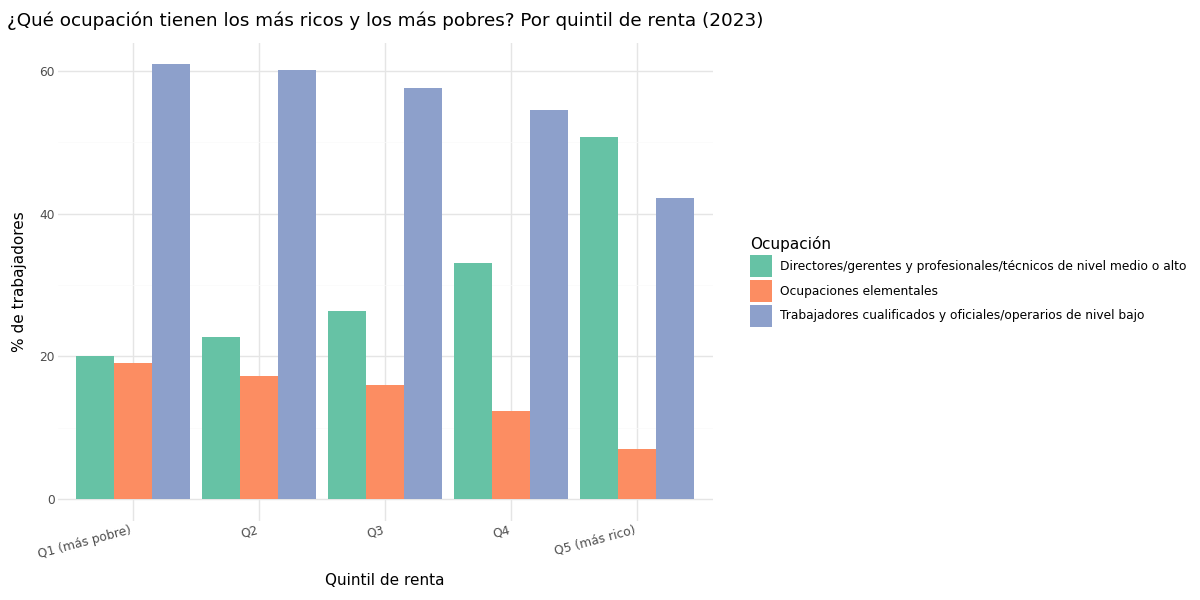
\includegraphics[width=\textwidth]{images/grouped_ocupacion}
\caption{Distribución de trabajadores por categoría de ocupación y quintil de renta (2023).}
\end{figure}

Mismo esquema que el anterior, pero la variable de agrupación es la categoría de ocupación (CNO) en lugar del sector de actividad. Se incluyen las tres categorías más informativas desde el punto de vista de la desigualdad: directores/técnicos, trabajadores cualificados y ocupaciones elementales. Los colores siguen un esquema semafórico: verde para la ocupación de mayor renta, rojo para la de menor.

\section{Heatmap: evolución de la renta municipal 2021--2023}

\begin{figure}[H]
\centering
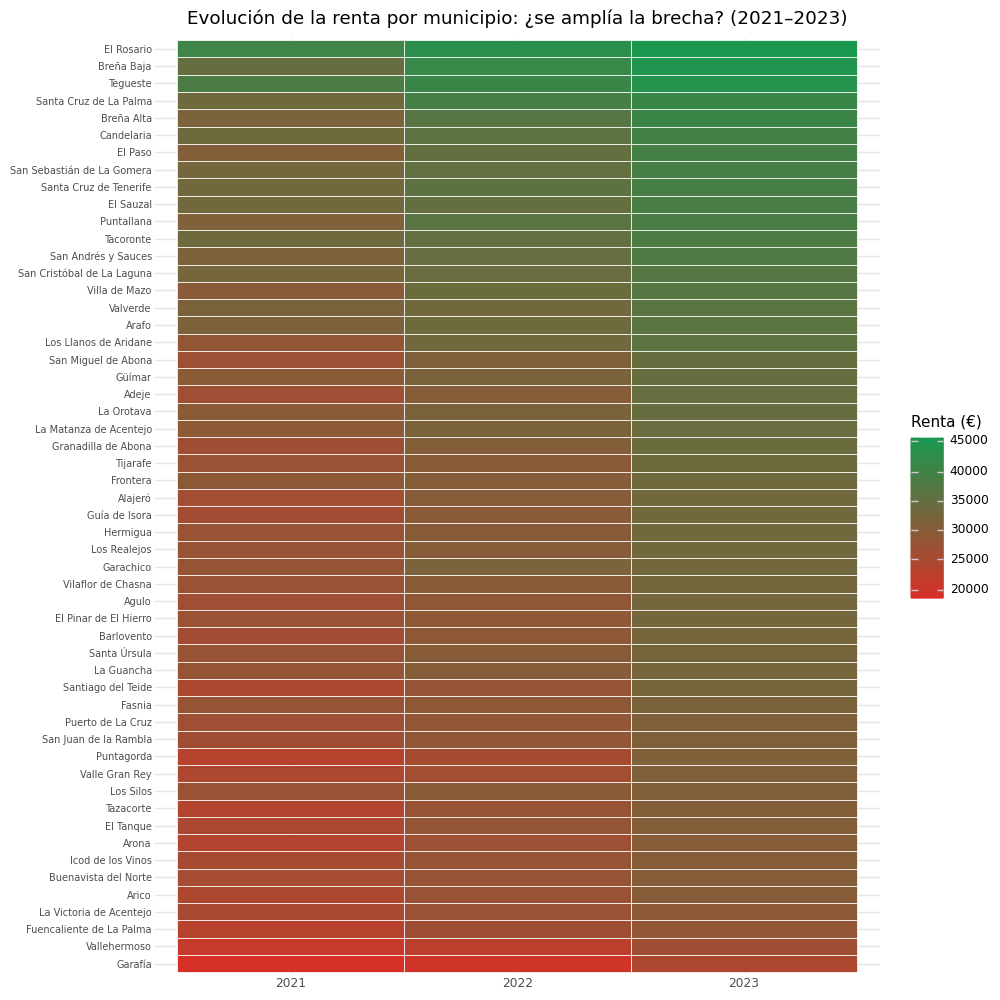
\includegraphics[width=0.85\textwidth]{images/heatmap}
\caption{Heatmap de renta media normalizada por municipio y año (2021--2023).}
\end{figure}

\begin{itemize}
  \item Datos: tabla con columnas municipio, año (2021, 2022, 2023) y renta\_norm (renta normalizada en [0,1] para poder comparar dentro del mismo municipio a lo largo del tiempo).
  \item Mapeos: x = año, y = municipio (ordenado por renta media), fill = renta\_norm.
  \item Geometrías: geom\_tile.
  \item Escalas: escala de color divergente (RdYlGn): rojo para renta baja, verde para renta alta.
  \item Coordenadas: cartesianas.
  \item Facetas: ninguna.
  \item Tema: texto del eje Y pequeño; leyenda de color a la derecha.
\end{itemize}

\section{Mapa interactivo: secciones censales}

\subsection{Técnica y datos}

El mapa es un mapa coroplético (choropleth) multicapa: cada polígono del territorio se colorea proporcionalmente al valor de una variable cuantitativa, y el usuario puede cambiar de capa mediante un control de capas. Los polígonos son las secciones censales de la provincia de Santa Cruz de Tenerife. Las tres capas disponibles son:

\begin{itemize}
  \item Renta neta media por hogar (euros), procedente del Atlas ADRH del INE (2023).
  \item Porcentaje de ingresos procedentes de prestaciones por desempleo, calculado a partir del fichero de distribución de renta (2023).
  \item Porcentaje de trabajadores en el sector Servicios sobre el total de asalariados, calculado a partir del fichero de actividad económica por sección censal (2023).
\end{itemize}

Los datos geométricos provienen de los ficheros GeoJSON del Instituto Geográfico Nacional (IGN), que delimitan las secciones censales a nivel de provincia. Estos polígonos se unen a cada dataframe mediante el código de sección censal de siete dígitos. La librería Folium genera el mapa como un documento HTML autónomo que envuelve una instancia de Leaflet.js, que gestiona las interacciones (zoom, paneo y tooltip al hover).

\subsection{Codificación visual}

Cada capa utiliza una paleta de color distinta para reforzar su significado temático:

\begin{itemize}
  \item Renta neta media: paleta divergente rojo-amarillo-verde (RdYlGn); el verde intenso indica renta alta y el rojo indica renta baja.
  \item Porcentaje de ingresos por desempleo: paleta secuencial verde claro a verde oscuro; el verde oscuro indica mayor dependencia de prestaciones.
  \item Porcentaje en Servicios: paleta secuencial naranja claro a naranja oscuro; la saturación indica mayor concentración en el sector.
\end{itemize}

En todas las capas, cada polígono incluye un tooltip que muestra el nombre del municipio y el valor de la variable al pasar el ratón, lo que permite identificar zonas de interés sin necesidad de una leyenda exhaustiva.

\subsection{Diseño geoespacial vs. gramática de gráficos}

A diferencia de los gráficos de Plotnine, este mapa no se puede describir completamente con la gramática de Wilkinson porque la variable geométrica (posición y forma de cada polígono) ya viene codificada en los datos GeoJSON y no es un mapeo libre. El único mapeo estético en sentido estricto es el del color. Sin embargo, los principios de diseño se aplican igualmente:

\begin{itemize}
  \item Figura-Fondo: los polígonos coloreados destacan sobre el tile base neutro (CartoDB Positron).
  \item Punto Focal: los clusters de color intenso atraen la atención y permiten identificar de inmediato las zonas extremas de cada variable.
  \item Proximidad: las secciones censales del mismo municipio son polígonos adyacentes, por lo que la homogeneidad de color dentro de un municipio se percibe sin etiquetas.
\end{itemize}

El mapa es la única visualización del proyecto en la que la dimensión espacial es el canal principal de codificación, lo que lo hace imprescindible para comunicar patrones de segregación residencial que no son perceptibles en los gráficos estadísticos.


% =============================================================================
\chapter{Principios de diseño y gestalt}
% =============================================================================

En la siguiente tabla se recoge para cada visualización qué principios de la gestalt o de diseño de visualización justifican las decisiones de codificación tomadas.

\begin{table}[H]
\centering
\small
\begin{tabular}{lp{4cm}p{7cm}}
\toprule
Gráfico & Principio(s) & Justificación \\
\midrule
Lollipop ranking & Figura-Fondo, Punto Focal & La línea delgada reduce el ruido visual (figura-fondo); el punto actúa como elemento focal que guía la lectura del valor preciso. \\
\addlinespace
Histograma renta & Proximidad, Figura-Fondo & Los bins adyacentes que comparten rango se perciben como grupo; el fondo blanco realza la distribución. \\
\addlinespace
Waterfall fuentes & Continuidad, Parte-Todo & Las barras encadenadas crean una línea de acumulación continua que comunica la composición del total; cada segmento es una parte del 100\%. \\
\addlinespace
Waterfall actividades & Continuidad, Parte-Todo & Mismo principio; la dominancia del sector servicios se percibe inmediatamente por la anchura relativa. \\
\addlinespace
Diverging bar género & Destino Común, Simetría & Las barras que se extienden hacia lados opuestos convergen en el eje de paridad; la simetría rota evidencia el desequilibrio. \\
\addlinespace
Box plots (islas) & Distribución, Punto Focal & La caja muestra la distribución completa; la mediana como línea central actúa de punto focal para la comparación entre municipios. \\
\addlinespace
Scatter & Correlación, Destino Común & Los puntos que forman una nube orientada negativamente señalan un destino común: a más educación elemental, menor renta. \\
\addlinespace
Grouped bar quintiles & Magnitud, Proximidad & Las barras agrupadas permiten comparar magnitudes entre quintiles; la proximidad física de las barras del mismo quintil facilita la comparación intragrupo. \\
\addlinespace
Grouped bar ocupación & Magnitud, Proximidad & Mismo principio aplicado a las categorías de ocupación. \\
\addlinespace
Heatmap & Cambio Temporal, Similitud & El color codifica magnitud; celdas del mismo tono se perciben como similares. La organización temporal en columnas facilita ver la evolución. \\
\addlinespace
Mapa interactivo & Figura-Fondo, Punto Focal & El gradiente de color sobre fondo neutro enfoca la atención en las diferencias espaciales de renta. \\
\bottomrule
\end{tabular}
\caption{Principios de diseño y gestalt por visualización.}
\end{table}


% =============================================================================
\chapter{Arquitectura DataOps con Dagster}
% =============================================================================

\section{Motivación}

El proyecto adopta una arquitectura DataOps basada en Dagster para automatizar la generación de los gráficos de forma reproducible, trazable y con garantías de calidad. Dagster organiza el trabajo como un grafo dirigido acíclico (DAG) de assets: cada función decorada con @asset declara explícitamente sus dependencias de datos, lo que permite al orquestador determinar el orden de ejecución y recalcular sólo los assets afectados por un cambio.

\section{Grafo de assets}

El pipeline se estructura en cuatro capas:

\begin{enumerate}
  \item Carga (*\_load): lectura de los datos crudos desde la API del INE o desde ficheros CSV en caché.
  \item Limpieza (*\_clean): normalización de tipos, filtrado de nulos y codificación de variables.
  \item Datos analíticos (data\_*): transformaciones específicas para cada gráfico (agrupaciones, pivotados, cálculos de quintiles, etc.).
  \item Visualizaciones (ranking\_municipios, hist\_renta, fuentes\_ingresos, ...): generación del archivo PNG o HTML final.
\end{enumerate}

\begin{lstlisting}[caption={Cadena de dependencias en Dagster (extracto).}]
rentamedia_load
    -> rentamedia_clean
        -> data_renta_municipio
            -> ranking_municipios   # PNG
        -> data_hist_renta
            -> hist_renta           # PNG
        -> data_boxplot_intramunicipal
            -> boxplot_intramunicipal  # 4 x PNG
        -> data_heatmap_renta
            -> heatmap_renta        # PNG
\end{lstlisting}

\section{Generación de código con IA y caché de prompts}

Los assets de visualización no contienen el código de Plotnine directamente. En su lugar, cada asset llama a la función auxiliar render\_ia\_viz, que:

\begin{enumerate}
  \item Calcula el hash MD5 del prompt de la visualización (almacenado en sources/*.hash).
  \item Si el hash ha cambiado, invoca la API de Claude para generar el código Python de la función generar\_plot(df) y lo guarda en scripts/*.py.
  \item Carga el módulo generado dinámicamente, llama a generar\_plot(df) con los datos del asset, y guarda el resultado como PNG.
\end{enumerate}

Este mecanismo garantiza que el código generado por la IA sea determinista: si el prompt no ha cambiado, se reutiliza el código en caché sin hacer ninguna llamada a la API. Sólo cuando el prompt se modifica (porque queremos un gráfico diferente) se regenera el script.

\begin{lstlisting}[caption={Función auxiliar de renderizado con caché de prompts.}]
def render_ia_viz(context, code: str, df, output_path: str,
                  width=10, height=6):
    namespace = {}
    exec(compile(code, "<ia_viz>", "exec"), namespace)
    plot = namespace["generar_plot"](df)
    plot.save(output_path, width=width, height=height, dpi=150)
    context.log.info(f"Guardado: {output_path}")
\end{lstlisting}

\begin{lstlisting}[caption={Patrón de asset con caché de prompt hash.}]
@asset
def ranking_municipios(context, prompt_ranking, data_renta_municipio):
    script_path = os.path.join(SOURCES_DIR, "ranking_municipios.py")
    hash_path   = os.path.join(SOURCES_DIR, "ranking_municipios.hash")
    prompt_hash = hashlib.md5(prompt_ranking.encode()).hexdigest()

    if not os.path.exists(hash_path) or \
       open(hash_path).read().strip() != prompt_hash:
        code = llamar_api_ia(prompt_ranking)
        with open(script_path, "w") as f:
            f.write(code)
        with open(hash_path, "w") as f:
            f.write(prompt_hash)

    with open(script_path) as f:
        code = f.read()

    output_path = "plots/renta/ranking_municipios.png"
    render_ia_viz(context, code, data_renta_municipio,
                  output_path, width=12, height=14)
    return output_path
\end{lstlisting}


% =============================================================================
\chapter{Checks de calidad de assets}
% =============================================================================

Cada asset importante cuenta con uno o más asset checks implementados en lab\_renta\_checks.py. Los checks son funciones decoradas con @asset\_check que devuelven un AssetCheckResult con un campo passed y metadatos adicionales.

\section{Clasificación de los checks}

\subsection{Checks de carga (integridad básica)}

\begin{table}[H]
\centering
\small
\begin{tabular}{lp{8cm}}
\toprule
Check & Qué verifica \\
\midrule
test\_rentamedia\_no\_nulos & Porcentaje de nulos en OBS\_VALUE < 5\% \\
test\_actividad\_sectores\_completos & Los 5 sectores de actividad económica están presentes \\
test\_ingresos\_fuentes\_completas & Las 5 fuentes de ingresos están presentes \\
\bottomrule
\end{tabular}
\caption{Checks de integridad en los assets de carga.}
\end{table}

\subsection{Checks de limpieza}

\begin{table}[H]
\centering
\small
\begin{tabular}{lp{8cm}}
\toprule
Check & Qué verifica \\
\midrule
test\_rentamedia\_rango\_valores & Renta neta en [3.000 euros, 200.000 euros]: rango razonable para España \\
test\_rentamedia\_cobertura\_temporal & Los años 2021, 2022 y 2023 están presentes \\
test\_ingresos\_conversion\_decimal & OBS\_VALUE en [0, 100] tras conversión de porcentajes \\
test\_ocupacion\_categorias & <= 10 categorías de ocupación (límite cognitivo de visualización) \\
\bottomrule
\end{tabular}
\caption{Checks sobre los assets de limpieza.}
\end{table}

\subsection{Checks analíticos}

Estos checks validan los supuestos narrativos del proyecto: si fallan, la historia que cuentan los gráficos pierde sustento estadístico.

\begin{table}[H]
\centering
\small
\begin{tabular}{lp{7.5cm}}
\toprule
Check & Qué verifica \\
\midrule
test\_cobertura\_municipios & Al menos 40 de los 54 municipios tienen datos de renta \\
test\_punto\_focal\_renta & Ratio renta máxima / mínima >= 1.5 (la desigualdad es suficiente para ser narrativa) \\
test\_hist\_dispersion & Coeficiente de variación de la renta > 0.15 (el histograma es informativo) \\
test\_waterfall\_suma\_100 & Las 5 fuentes de ingresos suman aprox. 100\% \\
test\_piramide\_categorias & El dataset tiene columna desviacion y >= 2 categorías \\
test\_waterfall\_actividades\_suma\_100 & Los 4 sectores CNAE suman aprox. 100\% \\
test\_boxplot\_cobertura & El boxplot tiene >= 40 municipios y >= 200 secciones censales \\
test\_scatter\_correlacion\_negativa & Correlación entre \% elementales y renta < -0.1 \\
test\_quintiles\_completos & 5 quintiles y >= 3 sectores de actividad \\
test\_ocupacion\_quintiles\_completos & 5 quintiles y >= 2 categorías de ocupación \\
test\_heatmap\_tres\_anios & El heatmap cubre los 3 años y >= 40 municipios \\
\bottomrule
\end{tabular}
\caption{Checks analíticos que validan los supuestos narrativos del proyecto.}
\end{table}

\subsection{Checks de integridad de archivos generados}

Para cada PNG generado existe un check que verifica que el archivo existe y tiene un tamaño mayor a 5 KB (lo que descarta archivos vacíos o corrompidos):

\begin{lstlisting}[caption={Función auxiliar compartida por todos los checks de archivo.}]
def _check_file(path, description, gestalt, min_size=5000):
    exists = os.path.exists(path)
    size   = os.path.getsize(path) if exists else 0
    return AssetCheckResult(
        passed=bool(exists and size > min_size),
        metadata={
            "path":    MetadataValue.path(path),
            "size_kb": MetadataValue.float(size / 1024),
            "description": description,
            "gestalt": gestalt,
        }
    )
\end{lstlisting}

% =============================================================================
\chapter{Dashboard interactivo}
% =============================================================================

El dashboard de Streamlit (dashboard.py) agrupa los catorce gráficos del proyecto junto con el mapa interactivo.

\section{Estructura y narrativa}

El dashboard se divide en seis secciones accesibles desde un menú de radio en la barra lateral (st.sidebar). El orden de las secciones refleja el orden lógico del análisis: primero el contexto espacial (mapa), luego la distribución general de la renta, después la composición económica, a continuación los patrones de desigualdad y género, luego el detalle intramunicipal y finalmente la relación con el nivel educativo y los quintiles.

\begin{table}[H]
\centering
\small
\begin{tabular}{lp{4.5cm}p{5.5cm}}
\toprule
Sección & Visualizaciones & Pregunta que responde \\
\midrule
Mapa interactivo & Mapa coroplético Folium & ?`Dónde están las zonas ricas y pobres? \\
\addlinespace
Distribución de la renta & Lollipop ranking, histograma & ?`Cuánta diferencia hay entre municipios? \\
\addlinespace
Composición económica & Waterfall fuentes, waterfall actividades & ?`De qué viven los habitantes? \\
\addlinespace
Desigualdad y género & Diverging bar & ?`Se reparte igual el trabajo precario? \\
\addlinespace
Desigualdad intramunicipal & 4 box plots (uno por isla) & ?`Cuánta heterogeneidad hay dentro de cada municipio? \\
\addlinespace
Educación y quintiles & Scatter, grouped bars & ?`Qué perfil educativo y laboral tienen los más ricos? \\
\bottomrule
\end{tabular}
\caption{Secciones del dashboard y preguntas que responden.}
\end{table}

Cada sección incluye un bloque de texto introductorio que contextualiza la visualización y un recuadro de conclusión (insight box) con el hallazgo principal. Ambos elementos se renderizan mediante st.markdown con HTML personalizado para controlar el estilo visual sin depender del tema por defecto de Streamlit.

\section{Integración del mapa interactivo}

La principal dificultad técnica del dashboard es incrustar el mapa Folium, que es un fichero HTML autónomo con JavaScript, dentro de una aplicación Streamlit. La solución es leer el HTML generado y pasarlo a st.components.v1.html, que crea un iframe en el que el navegador ejecuta el código Leaflet.js del mapa:

\begin{lstlisting}[caption={Incorporación del mapa Folium en Streamlit.}]
def show_map():
    with open("plots/secciones_map.html", "r") as f:
        html = f.read()
    st.components.v1.html(html, height=600, scrolling=False)
\end{lstlisting}

El mapa funciona con todas sus capacidades interactivas (zoom, paneo, tooltip al hover) dentro del iframe. La altura se fija en 600 píxeles para que quepa en una pantalla de resolución estándar sin necesidad de hacer scroll dentro del componente.

\section{Navegación y estilo}

La navegación lateral usa st.radio para listar las seis secciones. Al seleccionar una sección, Streamlit re-ejecuta el script y la función correspondiente renderiza el contenido. Los gráficos estáticos se muestran con st.image, que los escala al ancho de la columna de contenido.

El estilo visual se personaliza con CSS inyectado mediante st.markdown con unsafe\_allow\_html=True. Se definen dos clases: caption-box (borde azul a la izquierda, para las descripciones de contexto) e insight-box (borde amarillo a la izquierda, para los hallazgos principales). Esto mantiene la coherencia visual entre secciones sin necesidad de imágenes decorativas.

\section{Arranque}

El dashboard se lanza en el puerto 8501 para no interferir con otras aplicaciones que puedan usar el puerto 8080 o el 80:

\begin{lstlisting}[language=bash,caption={Arranque del dashboard.}]
streamlit run dashboard.py --server.port 8501
\end{lstlisting}

Una vez en marcha, la aplicación queda disponible en http://localhost:8501. Streamlit recarga automáticamente el dashboard cada vez que se guarda dashboard.py, lo que facilita iterar sobre el diseño sin reiniciar el servidor manualmente.


% =============================================================================
\chapter*{Apéndice: Prompts de generación de visualizaciones}
\addcontentsline{toc}{chapter}{Apéndice: Prompts de generación de visualizaciones}
% =============================================================================

Este apéndice recoge los prompts utilizados para que el modelo de lenguaje generase el código de cada visualización. Los prompts están diseñados para referenciar explícitamente los conceptos de la gramática de gráficos y las recomendaciones de diseño de la asignatura, de modo que el código generado siga los mismos principios que se estudian.

\section*{Consideraciones de diseño de los prompts}

Cada prompt incluye los siguientes elementos:

\begin{itemize}
  \item Tipo de gráfico y justificación: se indica el tipo de geometría (geom\_*) y por qué es adecuado para los datos (por ejemplo, "un lollipop evita la saturación visual de un gráfico de barras sin perder precisión").
  \item Mapeos estéticos explícitos: se especifica qué variable va en qué aes(), siguiendo la terminología de la gramática de gráficos.
  \item Transformaciones de coordenadas: cuando se requiere coord\_flip(), se indica explícitamente junto con el patrón correcto (x=categórica, y=numérica).
  \item Principios de gestalt: se mencionan los principios que debe activar el gráfico (por ejemplo, "punto focal en la cabeza del lollipop", "continuidad en la línea acumulada del waterfall").
  \item Recomendaciones de diseño: se incluyen instrucciones sobre paletas de colores semánticas, límite de categorías, ordenación por valor, etc.
\end{itemize}

\section*{Evaluación de los prompts}

Los prompts cumplen las siguientes condiciones de calidad:

\begin{enumerate}
  \item Referencian la gramática de gráficos: todos los prompts nombran explícitamente aes(), geom\_*, scale\_*, coord\_* y theme\_*.
  \item Referencian principios de diseño: al menos un principio de gestalt o de diseño de visualización se menciona en cada prompt.
  \item Especifican el schema de datos: cada prompt describe las columnas del dataframe de entrada (nombres y tipos) para que el modelo no haga suposiciones.
  \item Incluyen restricciones de calidad: se indica el formato de salida (función generar\_plot(df) que devuelve un objeto ggplot), el estilo de tema y las restricciones de accesibilidad.
\end{enumerate}

\section*{Prompts seleccionados}

\subsection*{Prompt: ranking de municipios (lollipop)}

\begin{lstlisting}[language={},caption={Prompt para el lollipop de ranking.}]
Genera una función generar_plot(df) que cree un lollipop chart con
plotnine. El dataframe df tiene columnas: municipio (str), renta_media
(float), isla (str).

Mapeos aes(): x=municipio (ordenado por renta_media de menor a mayor),
y=renta_media, color=isla. Usa geom_segment desde ymin=0 hasta yend
y geom_point para la cabeza. Aplica coord_flip() para que los nombres
de municipio se lean horizontalmente. Usa theme_minimal() y etiquetas
del eje Y en formato de miles de euros.

Principios de gestalt: Figura-Fondo (línea delgada minimiza el ruido visual),
Punto Focal (geom_point guía la lectura del valor).
\end{lstlisting}

\subsection*{Prompt: diverging bar de género en ocupaciones}

\begin{lstlisting}[language={},caption={Prompt para el diverging bar de brecha de género.}]
Genera una función generar_plot(df) con plotnine. El dataframe tiene
columnas: ocupacion (str), desviacion (float, negativo=mayoría
masculina, positivo=mayoría femenina), mayoria (str).

Mapeos: x=ocupacion (pd.Categorical ordenado por desviacion),
y=desviacion, fill=mayoria. Usa geom_col(width=0.6) + coord_flip() +
geom_hline(yintercept=0). IMPORTANTE: x debe ser la variable categórica
y y la numérica, no al revés. Usa scale_fill_manual con azul para
"Más hombres" y rojo para "Más mujeres" (convención de género).
Formato del eje Y: etiquetas con signo (+/-) y símbolo %.

Principios: Destino Común (las barras de categorías masculinizadas
apuntan en la misma dirección), Simetría (la asimetría real contrasta
con la simetría esperada en la paridad).
\end{lstlisting}

\subsection*{Prompt: box plots intramunicipal}

\begin{lstlisting}[language={},caption={Prompt para el box plot de desigualdad intramunicipal.}]
Genera una función generar_plot(df) con plotnine. El dataframe tiene
columnas: municipio (str), renta_neta (float), isla (str). El dataframe
ya viene filtrado para una sola isla.

Ordena los municipios por renta_neta mediana (usa pd.Categorical con
las categorías ordenadas). Mapeos: x=municipio, y=renta_neta.
Geometría: geom_boxplot con outlier_size=0.8 para no saturar. Aplica
coord_flip(). El título debe incluir el nombre de la isla (usa
df['isla'].iloc[0]). Usa theme_minimal() con legend_position='none'.

Principios: Distribución (la caja muestra varianza intramunicipal),
Punto Focal (la mediana como línea central del boxplot).
\end{lstlisting}

\subsection*{Prompt: grouped bar por quintiles de actividad}

\begin{lstlisting}[language={},caption={Prompt para el grouped bar de actividad por quintil.}]
Genera una función generar_plot(df) con plotnine. El dataframe tiene
columnas: quintil (int, 1-5), actividad (str, sector CNAE), pct (float).

Convierte quintil a str antes de usarlo. Mapeos: x=quintil, y=pct,
fill=actividad. Geometría: geom_col(position='dodge'). Usa
theme_minimal(). Las barras deben estar agrupadas (dodge), no apiladas.
Eje Y en porcentaje.

Principios: Magnitud (la altura de las barras codifica proporción),
Proximidad (las barras del mismo quintil se perciben como grupo).
\end{lstlisting}

\bigskip

\noindent Los prompts completos para todos los gráficos están almacenados en los assets prompt\_* del archivo lab\_renta.py y en los ficheros de caché sources/*.hash.


% =============================================================================
% Bibliografía
% =============================================================================

\begin{thebibliography}{9}

\bibitem{wilkinson2005}
Wilkinson, L. (2005). The Grammar of Graphics (2nd ed.). Springer.

\bibitem{plotnine}
Kibirige, H. et al. (2022). plotnine: A grammar of graphics for Python. Journal of Open Source Software, 7(74), 3523.

\bibitem{few2012}
Few, S. (2012). Show Me the Numbers: Designing Tables and Graphs to Enlighten (2nd ed.). Analytics Press.

\bibitem{cairo2016}
Cairo, A. (2016). The Truthful Art: Data, Charts, and Maps for Communication. New Riders.

\bibitem{dagster}
Elementl, Inc. (2023). Dagster: A data orchestrator for machine learning, analytics, and ETL. \url{https://dagster.io}

\bibitem{ine_adrh}
Instituto Nacional de Estadística (2024). Atlas de distribución de renta de los hogares. \url{https://www.ine.es/experimental/atlas/experimental_atlas.htm}

\end{thebibliography}

\end{document}
